\begin{figure}[t]
  \centering
  \caption{AGREE-Dog Evaluation Metrics and Convergence}
  \label{fig:agree-metrics-combined}

\begin{subfigure}{\textwidth}
    \centering
    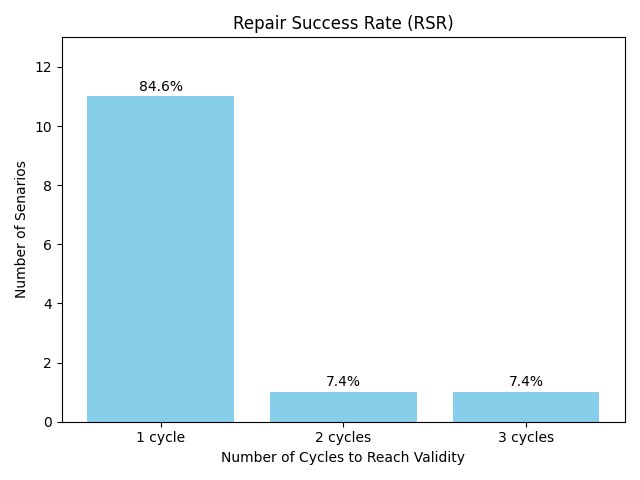
\includegraphics[width=0.6\linewidth]{repair-histogram.png}
    \caption{Repair cycles required to achieve system-wide validity.}
    \label{fig:repair-histogram}
  \end{subfigure}

  \vspace{1em}
  
  \begin{subfigure}{\textwidth}
    \centering
    \caption*{(b) Structural and Temporal Metrics Summary}
    \begin{minipage}{\textwidth}
      \centering
      \begin{tabular}{@{}p{0.48\textwidth} p{0.45\textwidth}@{}}
        \toprule
        \textbf{Metric} & \textbf{Result} \\
        \midrule
        \multicolumn{2}{l}{\textit{Structural Metrics}} \\
        System Validity & 100\% achieved for all test scenarios\\
        Repair Success Rate (RSR) & 11/13 (84.6\%) in 1 cycle; 1/13 in 2 cycles; 1/13 in 3 cycles \\
        Human Input Ratio (HpR) & $<$ 0.1\% of total tokens \\
        AGREE-Dog Generated Input & $>$ 99.9\% of total tokens \\
        Token Use (per test suite) & 4.8k, 5.5k, 22k tokens \\
        \addlinespace
        \multicolumn{2}{l}{\textit{Temporal Metrics}} \\
        Wall-Clock Time (WCT) & Mean: 2:09 min; Median: 1:39 min \\
        LLM Latency (per cycle) & Mean: 22 s; Range: 4--33 s \\
        \bottomrule
      \end{tabular}
    \end{minipage}
  \end{subfigure}

\end{figure}